% --------------------------------------------------------------
% This is all preamble stuff that you don't have to worry about.
% Head down to where it says "Start here"
% --------------------------------------------------------------
 
\documentclass[12pt]{article}
 
\usepackage[margin=1in]{geometry} 
\usepackage{amsmath,amsthm,amssymb}
\usepackage[margin=1in]{geometry} 
\usepackage{amsmath,amsthm,amssymb}
\usepackage[T1]{fontenc} %escribe lo del teclado
\usepackage[utf8]{inputenc} %Reconoce algunos símbolos
\usepackage{lmodern} %optimiza algunas fuentes
\usepackage{graphicx}
\graphicspath{ {images/} }
\usepackage{hyperref} % Uso de links
 
\newcommand{\N}{\mathbb{N}}
\newcommand{\Z}{\mathbb{Z}}
 
\newenvironment{theorem}[2][Theorem]{\begin{trivlist}
\item[\hskip \labelsep {\bfseries #1}\hskip \labelsep {\bfseries #2.}]}{\end{trivlist}}
\newenvironment{lemma}[2][Lemma]{\begin{trivlist}
\item[\hskip \labelsep {\bfseries #1}\hskip \labelsep {\bfseries #2.}]}{\end{trivlist}}
\newenvironment{exercise}[2][Exercise]{\begin{trivlist}
\item[\hskip \labelsep {\bfseries #1}\hskip \labelsep {\bfseries #2.}]}{\end{trivlist}}
\newenvironment{problem}[2][Problem]{\begin{trivlist}
\item[\hskip \labelsep {\bfseries #1}\hskip \labelsep {\bfseries #2.}]}{\end{trivlist}}
\newenvironment{question}[2][Question]{\begin{trivlist}
\item[\hskip \labelsep {\bfseries #1}\hskip \labelsep {\bfseries #2.}]}{\end{trivlist}}
\newenvironment{corollary}[2][Corollary]{\begin{trivlist}
\item[\hskip \labelsep {\bfseries #1}\hskip \labelsep {\bfseries #2.}]}{\end{trivlist}}

\newenvironment{solution}{\begin{proof}[Solution]}{\end{proof}}

\usepackage{listings}
\usepackage{color}

\definecolor{dkgreen}{rgb}{0,0.6,0}
\definecolor{gray}{rgb}{0.5,0.5,0.5}
\definecolor{mauve}{rgb}{0.58,0,0.82}

\lstset{
  language=Java,
  aboveskip=3mm,
  belowskip=3mm,
  showstringspaces=false,
  columns=flexible,
  basicstyle={\small\ttfamily},
  numbers=none,
  numberstyle=\tiny\color{gray},
  keywordstyle=\color{blue},
  commentstyle=\color{dkgreen},
  stringstyle=\color{mauve},
  breaklines=true,
  breakatwhitespace=true,
  tabsize=3
}

\usepackage{enumitem}

\begin{document}
 
% --------------------------------------------------------------
%                         Start here
% --------------------------------------------------------------
 
\title{CS20B: HW 3}
\author{Nashir Janmohamed\\
Fall, 2019}

\maketitle
\section{Questions}
\begin{enumerate}
  \item Given the following method:
  \begin{lstlisting}
int exer (int num)
{
if ( num == 0)
  return 0;
else
  return num + exer (num + 1);
}
  \end{lstlisting}
  \begin{enumerate}[label=\Alph*]
    \item \textbf{Q.} Is there a constraint on the value that can be passed as an argument for this method to pass the smaller-caller test?
    \\\\
    \textbf{A.} Yes, the numbers must be less than or equal to 0. If they are positive integers, this method will never terminate, resulting in a StackOverflowException.
    \\
    \item \textbf{Q.} Is $exer(7)$ a valid call? If so, what is returned from the method?
    \\\\
    \textbf{A.} No it is not.
    \\
    \item \textbf{Q.} Is $exer(0)$ a valid call? If so, what is returned from the method?
    \\\\
    \textbf{A.} Yes it is. The method will return zero.
    \\
    \item \textbf{Q.} Is $exer(-5)$ a valid call? If so, what is returned from the method?
    \\\\
    \textbf{A.} Yes it is. The function will return (-5) + (-4) + (-3) + (-2) + (-1) + (0) == -15.
  \end{enumerate}
  \item
  You must assign the grades for a programming class. Right now the class is studying recursion, and students have been given this assignment: Write a recursive method sumValues that is passed an index into an array values of int (this array is accessible from within the sumValues method) and returns the sum of the values in the array between the location indicated by index and the end of the array. The argument will be between 0 and values.length inclusive. For example, given the configuration of values seen in Figure 1:
  
  \begin{figure}[!htb]
        \center{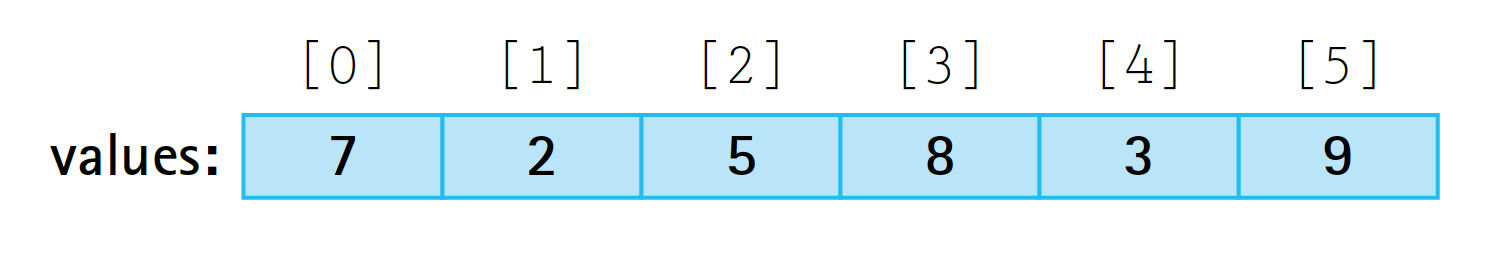
\includegraphics[width=11cm]
        {values.png}}
        \caption{\label{fig:values} Sample array values.}
\end{figure}
  
  then $sumValues(4)$ returns $12$ and $sumValues(0)$ returns $34$ (the sum of all the values in the array). You have received quite a variety of solutions. Grade the methods below. If the solution is incorrect, explain what the code actually does in lieu of returning the correct result. You can assume the array is ``full.'' You can assume a ``friendly'' user-the method is invoked with an argument between $0$ and $values.length$.
  \begin{enumerate}[label=\Alph*]
  \item \textbf{Q.}
    \begin{lstlisting}
int sumValues(int index)
{
  if (index == values.length)
    return 0;
  else
    return index + sumValues(index + 1);
}
    \end{lstlisting}
  \textbf{A.} This function has the right base case, but instead of summing the elements of values, it sums the values of the indexes for $indexes \in [index, values.length)$. This student should get $\frac{1}{2}$ points on this problem for getting the right base case but not correctly summing the values.
  \\
  \item \textbf{Q.}
    \begin{lstlisting}
int sumValues(int index)
{
  int sum = 0;
  for (int i = index; i < values.length; i++)
    sum = sum + values[i];
  return sum;
}
    \end{lstlisting}
  \textbf{A.} This function correctly sums the values from $[index, values.length)$, but it does it iteratively rather than recursively. This student should get $\frac{1}{4}$ points on this problem since they did not read the directions carefully enough, even though they provided a working implementation of the function.
  \\
  \item \textbf{Q.}
    \begin{lstlisting}
int sumValues(int index)
{
  if (index == values.length)
    return 0;
  else
    return 1 + sumValues(index + 1);
}
    \end{lstlisting}
  \textbf{A.} This function has the right base case, but instead of summing the elements of values, it sums the number of elements in the range of $[index, values.length)$. This student should get $\frac{1}{2}$ points on this problem for getting the right base case but not correctly summing the values.
  \\
  \item \textbf{Q.}
    \begin{lstlisting}
int sumValues(int index)
{
  return values[index] + sumValues(index + 1);
}
    \end{lstlisting}
  \textbf{A.} This function sums the elements of values recursively, but since it doesn't have a base case, it access values[values.length] which causes an ArrayOutOfBoundsException. This student should get $\frac{1}{2}$ points for writing the recursive part of the function correctly but not writing a base case.
  \\
  \item \textbf{Q.}
    \begin{lstlisting}
int sumValues(int index)
{
  if (index > values.length)
    return 0;
  else
    return values[index] + sumValues(index + 1);
}
    \end{lstlisting}
  \textbf{A.} This function sums the elements of values recursively, but the base case is wrong. The base case checks whether index > values.length, which will go out of bounds when index is equal to values.length which causes an ArrayOutOfBoundsException. This student should get $\frac{3}{4}$ points for writing the recursive part of the function correctly but not writing the correct base case.
  \\
  \item \textbf{Q.}
    \begin{lstlisting}
int sumValues(int index)
{
  if (index >= values.length)
    return 0;
  else
    return values[index] + sumValues(index + 1);
}
    \end{lstlisting}
  \textbf{A.} This function is perfect. It sums the elements recursively, and returns if index is greater than or equal to values.length. This student should get full points.
  \\
  \item \textbf{Q.}
    \begin{lstlisting}
int sumValues(int index)
{
  if (index < 0)
    return 0;
  else
    return values[index] + sumValues(index - 1);
}
    \end{lstlisting}
  \textbf{A.} This function is correct in that it sums the elements of vals, but instead of summing values in the range of $[index, values.length)$, it sums the values in the range of $[0, index]$. Even though the student provided a working recursive function, they clearly did not read the directions carefully enough, and so they should get $\frac{1}{4}$ points on this problem.
  \\
  \end{enumerate}
  \item Look at Figure 2. Explain the following:
\begin{figure}[!htb]
        \center{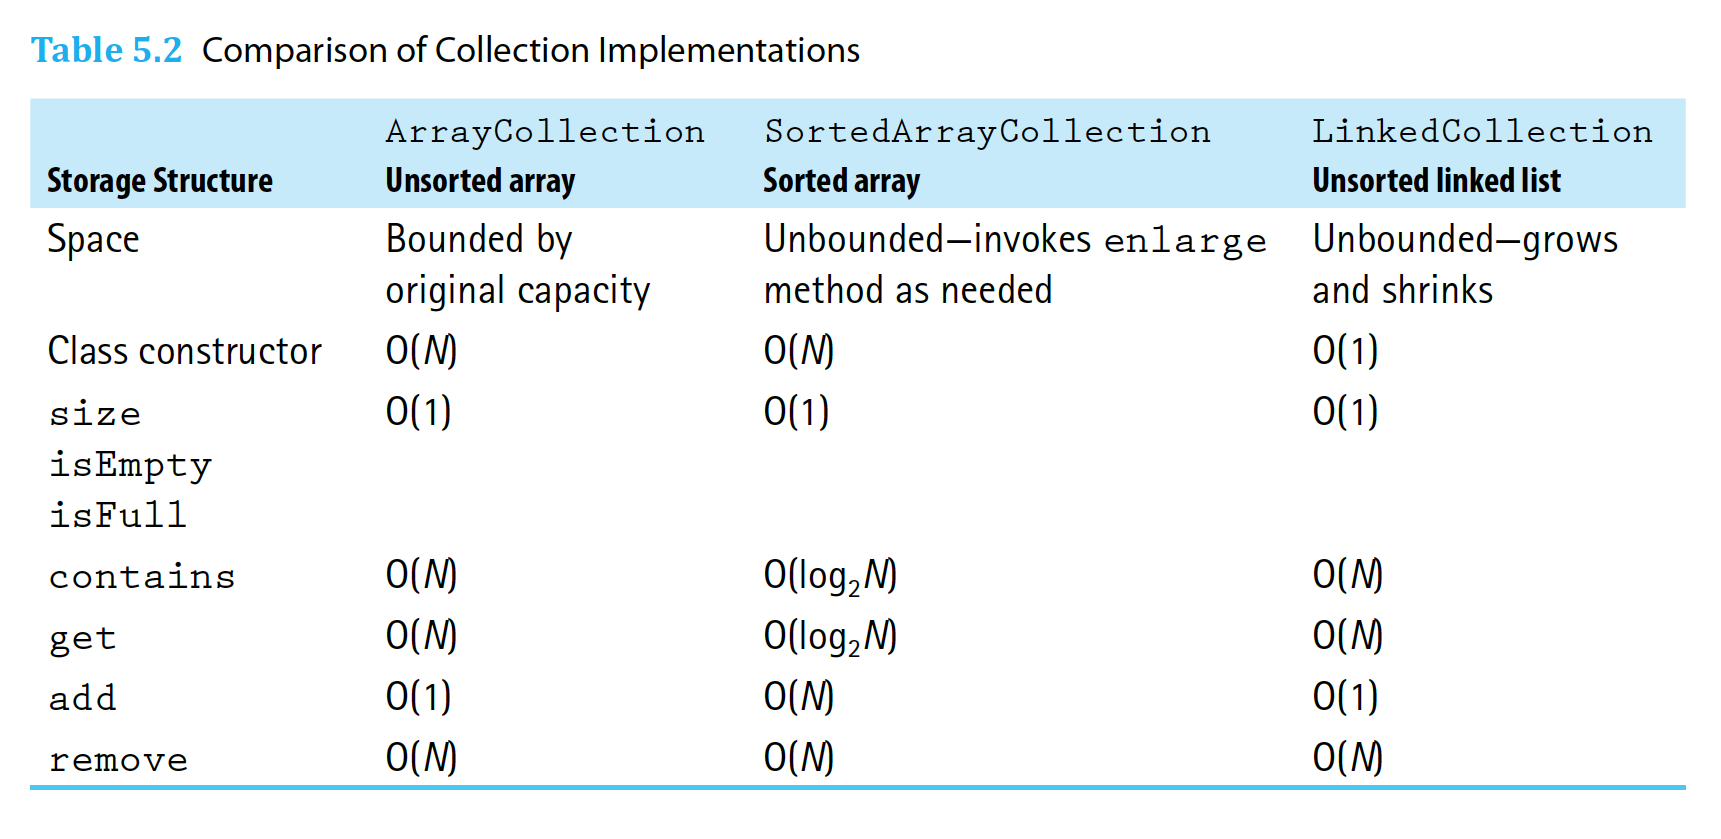
\includegraphics[width=11cm]
        {collection-comparisons.png}}
        \caption{\label{fig:collection-comparisons} Collection operation time complexity comparisons.}
\end{figure}

    \begin{enumerate}[label=\Alph*]
    \item \textbf{Q.} Why does SortedArrayCollection exhibit logarithmic time for contains and get methods?
    \\\\
     \textbf{A.} Since SortedArrayCollection is sorted, we can perform binary search on the elements of the array to determine whether or not a given element is in the collection (i.e. contains) or use binary search to get a particular element (i.e. get). Both of these can make use of a helper function called find() that returns the element if it exists in the collection, or null if it does not. Since the time complexity of binary search is $log_{2}(n)$, the time complexity of find (and therefore contains and get) is also logarithmic.
     \\
    \item \textbf{Q.} Why do ArrayCollection and LinkedCollection exhibit O(1) time for add (adding an element method), while SortedArrayCollection exhibits a worse O(N) time for the same method?
    \\\\
     \textbf{A.} When elements are added to ArrayCollection or LinkedCollection, the elements are added to the end, which doesn't take into account any particular ordering. The SortedArrayCollection must insert an element at a particular location $i$ in the array such that element at index $i-1$ has a value less than the inserted element and the element at index $i+1$ has a value greater than the inserted element (i.e. sortedColl.get(i-1).lessThan(sortedColl.get(i)) \&\& sortedColl.get(i+1).greaterThan(sortedColl.get(i))). In the worst case, an element to be inserted needs to be placed at the front of the array, in which case all elements must be shifted one element, which has a time complexity of O(N). Since big O notation considers the worst case, the insertion operation has a time complexity of O(N).
     \\
    \item \textbf{Q.} How is O(1) accomplished for size method for all of these collections in the table?
    \\\\
     \textbf{A.} The collection has an int field element called size that is incremented when items are added to the collection and decremented when items are removed from the collection. In essence, the size() method is just a getter for the size element, and getter methods (usually) operate in constant time.
     \\
  \end{enumerate}
  \item
    \begin{enumerate}[label=\Alph*]
    \item \textbf{Q.} Which method do we need to implement to check if the contents of our objects are the same?
    \\\\
     \textbf{A.} We need to implement the equals() method.
     \\
    \item \textbf{Q.} Write its signature.
    \\\\
     \textbf{A.} public boolean equals(Object obj);
     \\
    \item \textbf{Q.} Is it inherited from some class?
    \\\\
     \textbf{A.} Yes.
     \\
    \item \textbf{Q.} If yes, which one?
    \\\\
     \textbf{A.} It is inherited from the Object class.
     \\
  \end{enumerate}
  \item Based on the equals method for Circle objects defined in Section 5.4, ``Comparing Objects Revisited,'' what is the output of the following code sequence and \textbf{why}? Provide an answer for each of the eight printouts.
  \begin{lstlisting}
Circle c1 = new Circle(5);
Circle c2 = new Circle(5);
Circle c3 = new Circle(15);
Circle c4 = null;
  \end{lstlisting}
  \begin{enumerate}[label=\Alph*]
  \item \textbf{Q.}
  \begin{lstlisting}
System.out.println(c1 == c1);
  \end{lstlisting}
  \textbf{A.} This will output ``true''. When the equality operator ``=='' is used to compare two objects, it compares the address to which the references point. In this case, $c1$ is compared to itself, so this comparison will be true.
  \\
  \item \textbf{Q.}
  \begin{lstlisting}
System.out.println(c1 == c2);
  \end{lstlisting}
  \textbf{A.} This will output ``false''. Though $c1$ and $c2$ are initialized with the same value, $c1$ and $c2$ are both dynamically allocated memory on the stack, so they don't share the same memory address. Since the memory address are not the same, this comparison will be false.
  \\
  \item \textbf{Q.}
  \begin{lstlisting}
System.out.println(c1 == c3);
  \end{lstlisting}
  \textbf{A.} This will output ``false'' by the same reasoning as above.
  \\
  \item \textbf{Q.}
  \begin{lstlisting}
System.out.println(c1 == c4);
  \end{lstlisting}
  \textbf{A.} This will output ``false''. $c1$ is not null, so comparing it to null will output false.
  \\
  \item \textbf{Q.}
  \begin{lstlisting}
System.out.println(c1.equals(c1));
  \end{lstlisting}
  \textbf{A.} This will output ``true''. The equals method will return true if the object passed to the equals method is the same as calling object, which is true in this case.
  \\
  \item \textbf{Q.}
  \begin{lstlisting}
System.out.println(c1.equals(c2));
  \end{lstlisting}
  \textbf{A.} This will output ``true''. The equals method compares the radius of each Circle object, and since they are the same (i.e. both are passed the same initial value in the constructor), they are equal.
  \\
  \item \textbf{Q.}
  \begin{lstlisting}
System.out.println(c1.equals(c3));
  \end{lstlisting}
  \textbf{A.} This will output ``false''. The equals method compares the radius of each Circle object, and since they are different (i.e. c1's constructor is passed 5 while c3's constructor is passed 15), they are not equal.
  \\
  \item \textbf{Q.}
  \begin{lstlisting}
  System.out.println(c1.equals(c4));
  \end{lstlisting}
  \textbf{A.} This will output ``false''. The equals method will return false if the object passed to the equals method is null.
  \end{enumerate}
  \item Consider the following interfaces:
  \begin{lstlisting}
public interface Event {
  public void RSVP();
}
public interface PublicEvent extends Event {
  public void doSecurityCheck();
}
public interface PrivateEvent extends Event {
  public void checkIdentification();
}
public interface PartneredEvent extends Event {
  public void findPartner();
}
  \end{lstlisting}
  Which method(s) should implement a class
    \begin{enumerate}[label=\Alph*]
    \item \textbf{Q.} called Hockey that implements PublicEvent?
    \\\\
    \textbf{A.} Hockey must implement RSVP() and doSecurityCheck().
    \\
    \item \textbf{Q.} called Prom that implements PrivateEvent and PartneredEvent.
    \\\\
    \textbf{A.} Prom must implement RSVP(), checkIdentification(), and findPartner().
  \end{enumerate}
\end{enumerate}

% --------------------------------------------------------------
%     You don't have to mess with anything below this line.
% --------------------------------------------------------------
 
\end{document}